\documentclass{standalone}
\usepackage{amsmath}
\usepackage{bm}
\usepackage[dvipsnames]{xcolor}

\usepackage{tikz}
\usetikzlibrary{positioning,arrows.meta,backgrounds,shapes}
\usetikzlibrary{matrix}

\definecolor{train}{HTML}{00203f}
\definecolor{test}{HTML}{adefd1}
\definecolor{unused}{HTML}{bcbcbc}
\definecolor{validation}{HTML}{fb8b23}

\begin{document}

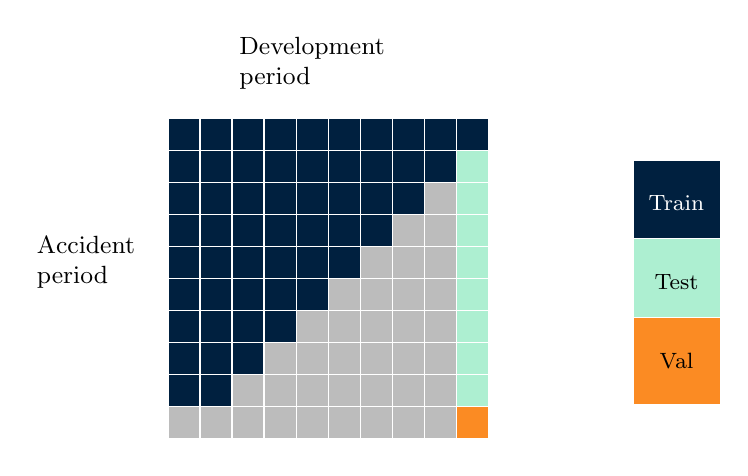
\begin{tikzpicture}[
    cell1/.style = {rectangle, fill=train, minimum size=.4cm, very thin, draw=white},
    cell2/.style = {rectangle, fill=unused, minimum size=.4cm, very thin, draw=white},
    cell3/.style = {rectangle, fill=test, minimum size=.4cm, very thin, draw=white},
    cell4/.style = {rectangle, fill=validation, minimum size=.4cm, very thin, draw=white},
]
    % triangle
    \matrix (triangle) [
        matrix of nodes, 
        nodes in empty cells, 
        in front of path, 
        ampersand replacement = \&, 
        xshift=4cm,
        yshift=-3cm
    ]
    {
        % row 1
        \node[cell1] {}; \&
        \node[cell1] {}; \&
        \node[cell1] {}; \&
        \node[cell1] {}; \&
        \node[cell1] (col5) {}; \&
        \node[cell1] {}; \&
        \node[cell1] {}; \&
        \node[cell1] {}; \&
        \node[cell1] {}; \&
        \node[cell1] {}; \\
        % row 2
        \node[cell1] {}; \&
        \node[cell1] {}; \&
        \node[cell1] {}; \&
        \node[cell1] {}; \&
        \node[cell1] {}; \&
        \node[cell1] {}; \&
        \node[cell1] {}; \&
        \node[cell1] {}; \&
        \node[cell1] {}; \&
        \node[cell3] {}; \\
        % row 3
        \node[cell1] {}; \&
        \node[cell1] {}; \&
        \node[cell1] {}; \&
        \node[cell1] {}; \&
        \node[cell1] {}; \&
        \node[cell1] {}; \&
        \node[cell1] {}; \&
        \node[cell1] {}; \&
        \node[cell2] {}; \&
        \node[cell3] {}; \\
        % row 4
        \node[cell1] {}; \&
        \node[cell1] {}; \&
        \node[cell1] {}; \&
        \node[cell1] {}; \&
        \node[cell1] {}; \&
        \node[cell1] {}; \&
        \node[cell1] {}; \&
        \node[cell2] {}; \&
        \node[cell2] {}; \&
        \node[cell3] {}; \\
        % row 5
        \node[cell1] {}; \&
        \node[cell1] {}; \&
        \node[cell1] {}; \&
        \node[cell1] {}; \&
        \node[cell1] {}; \&
        \node[cell1] {}; \&
        \node[cell2] {}; \&
        \node[cell2] {}; \&
        \node[cell2] (row5) {}; \&
        \node[cell3] {}; \\
        % row 6
        \node[cell1] {}; \&
        \node[cell1] {}; \&
        \node[cell1] {}; \&
        \node[cell1] {}; \&
        \node[cell1] {}; \&
        \node[cell2] {}; \&
        \node[cell2] {}; \&
        \node[cell2] {}; \&
        \node[cell2] {}; \&
        \node[cell3] {}; \\
        % row 7
        \node[cell1] {}; \&
        \node[cell1] {}; \&
        \node[cell1] {}; \&
        \node[cell1] {}; \&
        \node[cell2] {}; \&
        \node[cell2] {}; \&
        \node[cell2] {}; \&
        \node[cell2] {}; \&
        \node[cell2] {}; \&
        \node[cell3] {}; \\
        % row 8
        \node[cell1] {}; \&
        \node[cell1] {}; \&
        \node[cell1] {}; \&
        \node[cell2] {}; \&
        \node[cell2] {}; \&
        \node[cell2] {}; \&
        \node[cell2] {}; \&
        \node[cell2] {}; \&
        \node[cell2] {}; \&
        \node[cell3] {}; \\
        % row 9
        \node[cell1] {}; \&
        \node[cell1] {}; \&
        \node[cell2] {}; \&
        \node[cell2] {}; \&
        \node[cell2] {}; \&
        \node[cell2] {}; \&
        \node[cell2] {}; \&
        \node[cell2] {}; \&
        \node[cell2] {}; \&
        \node[cell3] {}; \\
        % row 10
        \node[cell2] {}; \&
        \node[cell2] {}; \&
        \node[cell2] {}; \&
        \node[cell2] {}; \&
        \node[cell2] {}; \&
        \node[cell2] {}; \&
        \node[cell2] {}; \&
        \node[cell2] {}; \&
        \node[cell2] {}; \&
        \node[cell4] {}; \\
    };

    % triangle labels
    \node [left of = row5, font=\small, align=left, xshift=-3.5cm] (xlabel) {Accident\\ period};
    \node [above of = col5, font=\small, align=left, yshift=-0.1cm] (ylabel) {Development\\ period};
    \node [cell1, right of = row5, xshift=2cm, yshift=.75cm,text=white, minimum size=1.1cm, font=\footnotesize, inner sep=5pt] (train) {Train};
    \node [cell3, below of = train, font=\footnotesize, minimum size=1.1cm, inner sep=5pt] (test) {Test};
    \node [cell4, below of = test, font=\footnotesize, minimum size=1.1cm, inner sep=5pt] (validation) {Val};

\end{tikzpicture}
\end{document}